\section{基于Zigzag映射矩阵的时间隐通道评估}
\label{chap:zigzag:results}
本节对基于Zigzag的时间隐通道进行评估,参照时间隐通道的构造指标要求,评估由抗检测能力、鲁棒性、传输性能及构建代价几个方面组成。其中,抗检测能力测试按照\nref{chap:analyze:statistical}提出的检测方法进行。

\subsection{评估环境及参数}
\label{chap:zigzag:results:environment}
该时间隐通道构建方法中,主要的参数为$L_{Codeword}$,其取值决定了传输性能水平,并对抗检测能力有显著影响。实验的测试场景,为\nref{chap:analyze:results}中表\nref{tab:3:capture-results}两种场景下的测试数据,在其基础上进行调制及解调测试,并对比调制前后的结果进行抗检测能力测试。

此外,在测试鲁棒性方面,为比较不同丢包率下的误码率水平,随机生成了丢包率在0.5\%、1\%、2\%、5\%、10\%共5种噪声。均匀分布的随机噪声,相比于连续丢包,对时间隐通道的影响更加显著。不同丢包率下的测试结果,可以有效体现时间隐通道的鲁棒性水平。

\insertTable{
	\begin{table}[]
      \centering
      \caption{基于Zigzag映射矩阵时间隐通道的参数取值}
      \label{tab:4:parameters}
          \begin{tabular*}{0.5\textwidth}{@{\extracolsep{\fill}}ccc}
            \toprule
            $L_{Codeword}$\ (bit) & $2^{L_{Codeword}}$ & 丢包率 \\
            \midrule
            7 & 128 & 0.781\% \\ 
            8 & 256 & 0.391\% \\ 
            9 & 512 & 0.195\% \\ 
            10 & 1024 & 0.098\% \\ 
            11 & 2048 & 0.049\% \\ 
            \bottomrule
          \end{tabular*}
    \end{table}
}

参照\nref{chap:analyze:result}的实验结果,两种场景下的$L_{Codeword}$取值如表\nref{tab:4:parameters},在基本能够通过测试的前提下进行其他测试。

\subsection{抗检测能力测试}
\label{chap:zigzag:results:undetectability}

按照\nref{chap:analyze:statistical}中提出的时间隐通道检测方法,对基于Zigzag映射矩阵的时间隐通道抗检测能力的评估,由IPD分布、突发丢包长度分布及区间丢包数分布组成,评估方式及参数保持一致。

\insertFigure{
	\begin{figure}
        \centering
        \subfigure[Excellent场景的CDF]{
            \label{fig:4:results:ipd:cdf:excellent}
            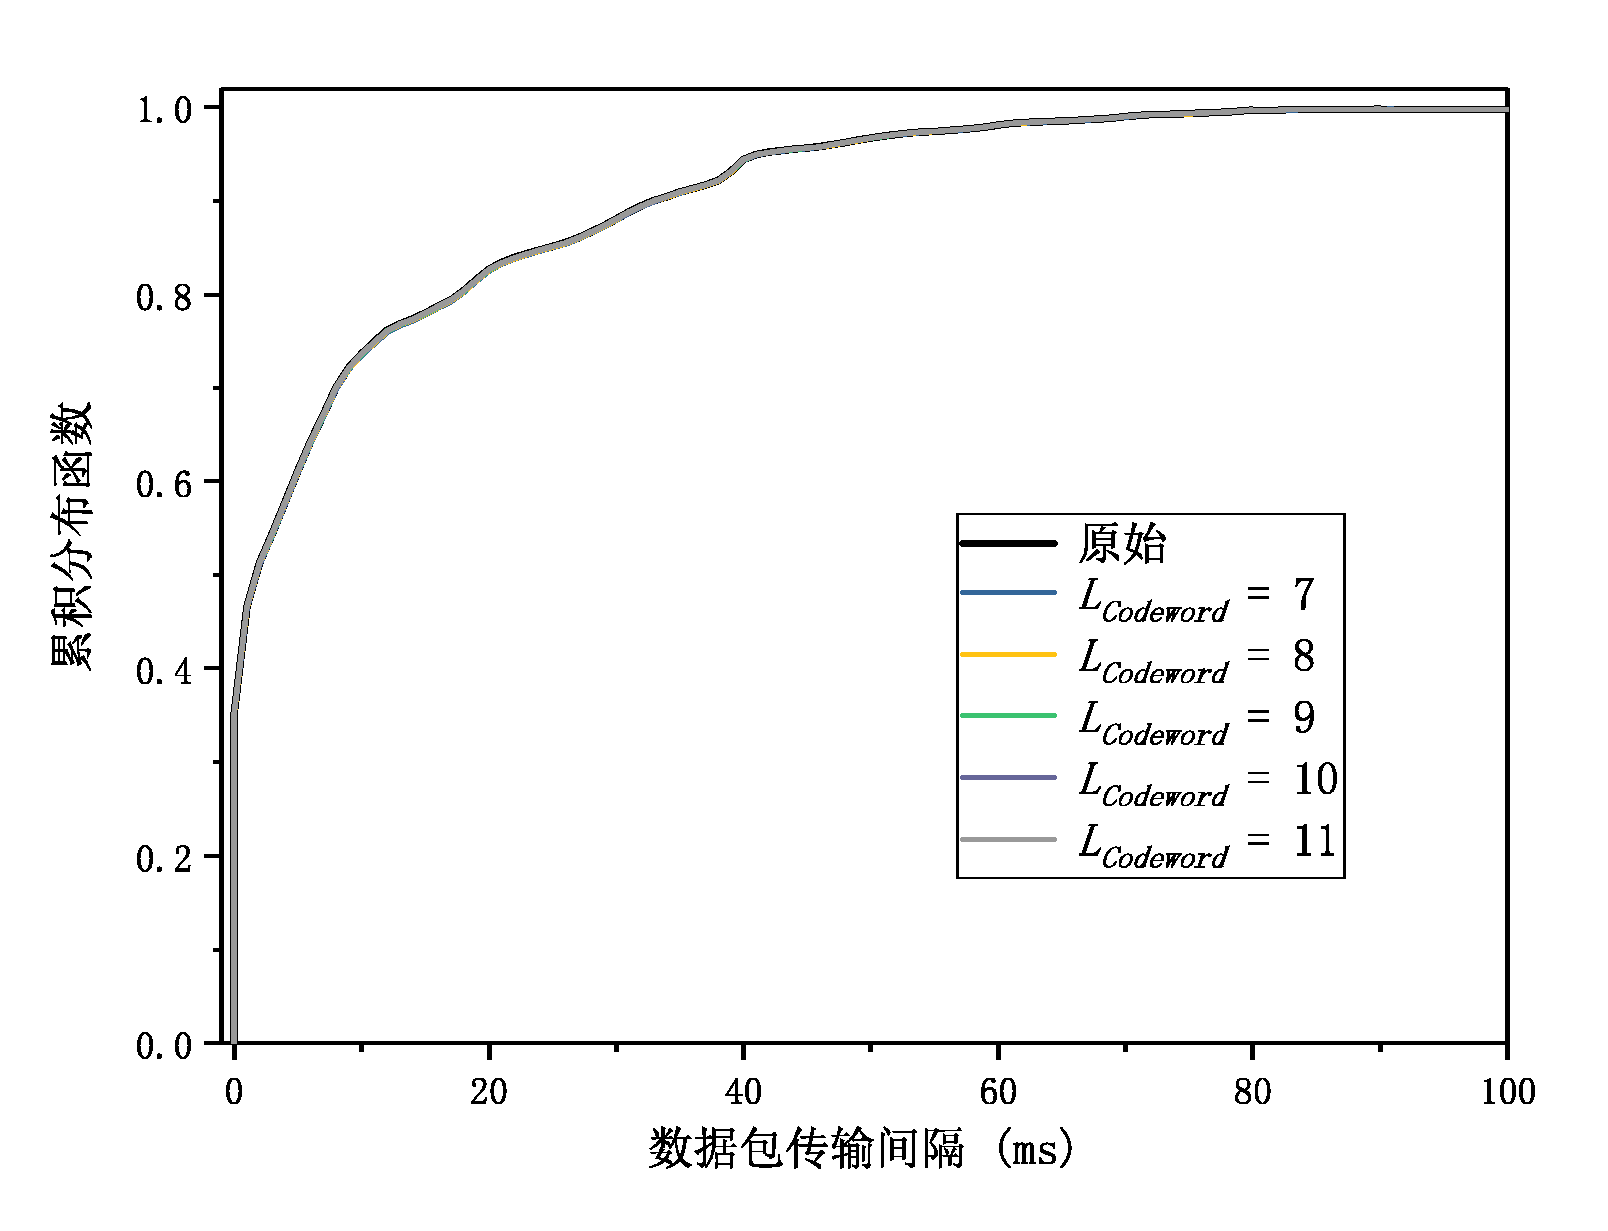
\includegraphics[width=0.48\textwidth]{chapters/chapter4/figures/ipd-cdf-excellent.pdf}
        }
        \subfigure[Good场景的CDF]{
            \label{fig:4:results:ipd:cdf:good}
            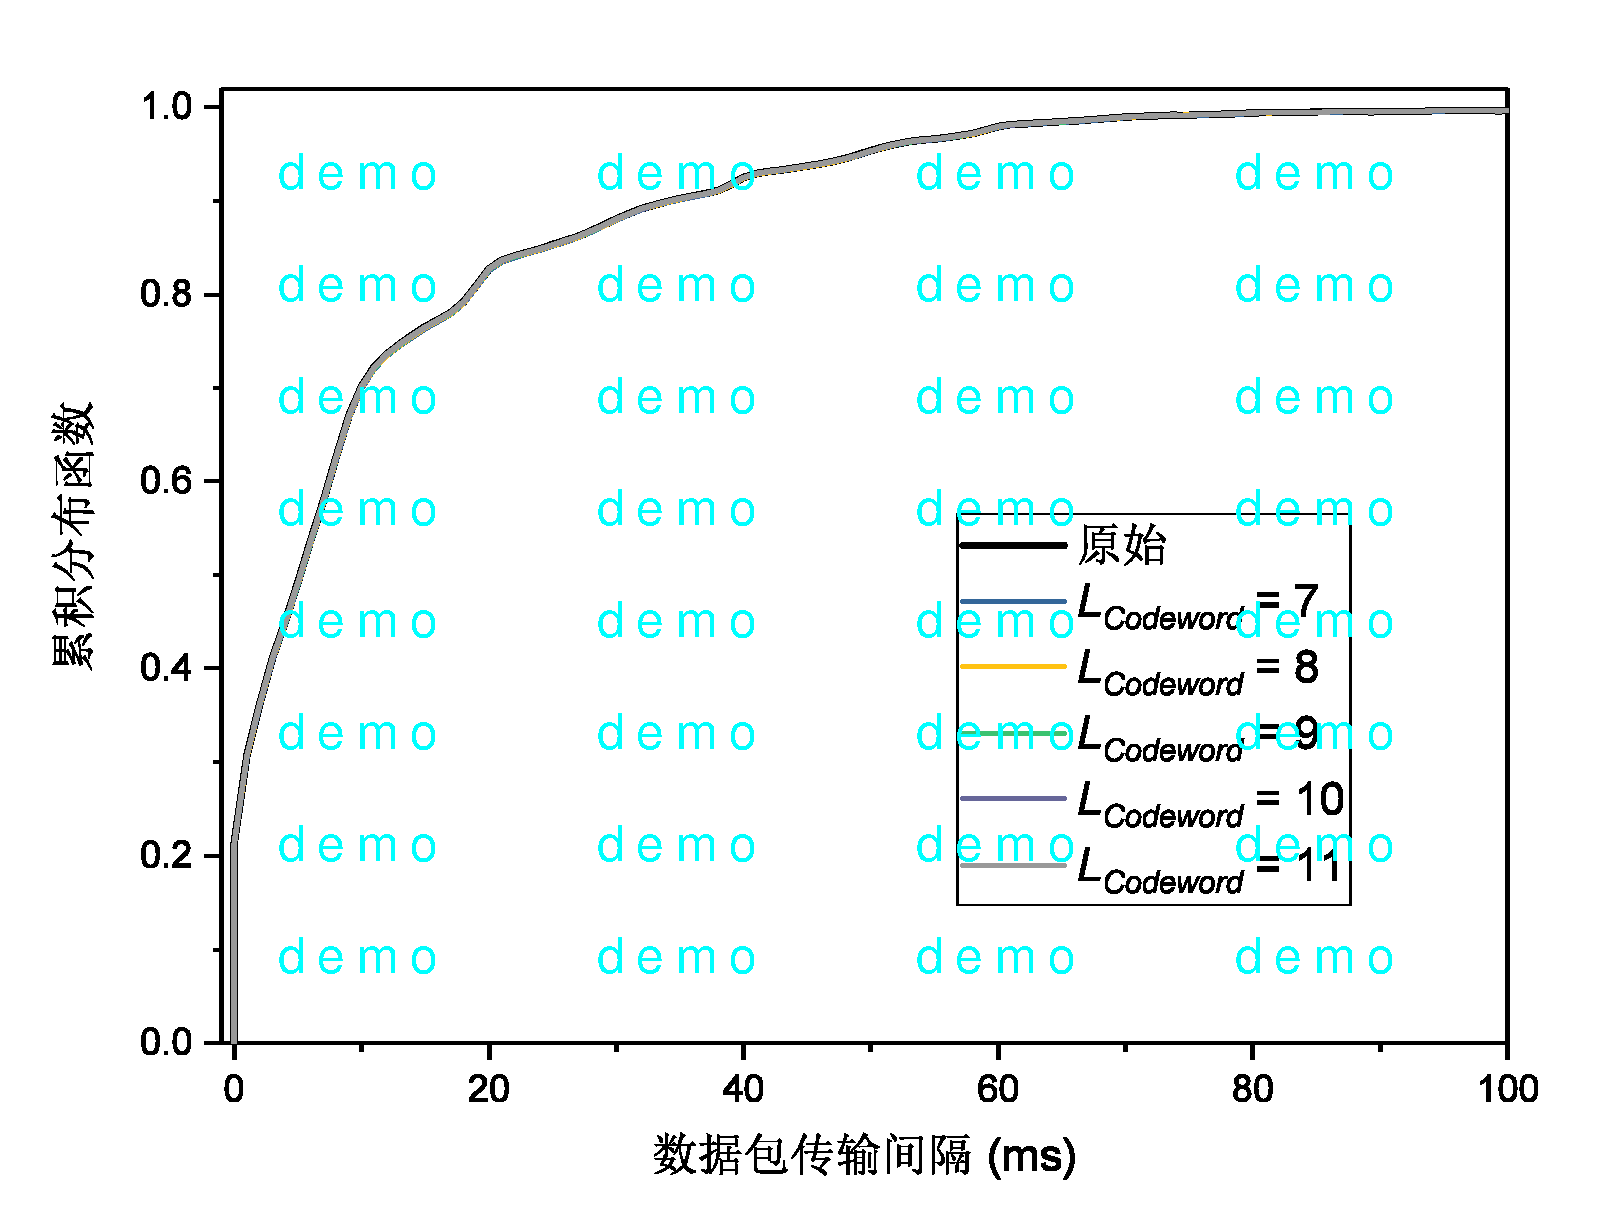
\includegraphics[width=0.48\textwidth]{chapters/chapter4/figures/ipd-cdf-good.pdf}
        }
        \caption{IPD分布的CDF曲线}
        \label{fig:4:results:ipd:cdf}
    \end{figure}
    
    \begin{figure}
        \centering
        \subfigure[Excellent场景的CDF]{
            \label{fig:4:results:burst:cdf:excellent}
            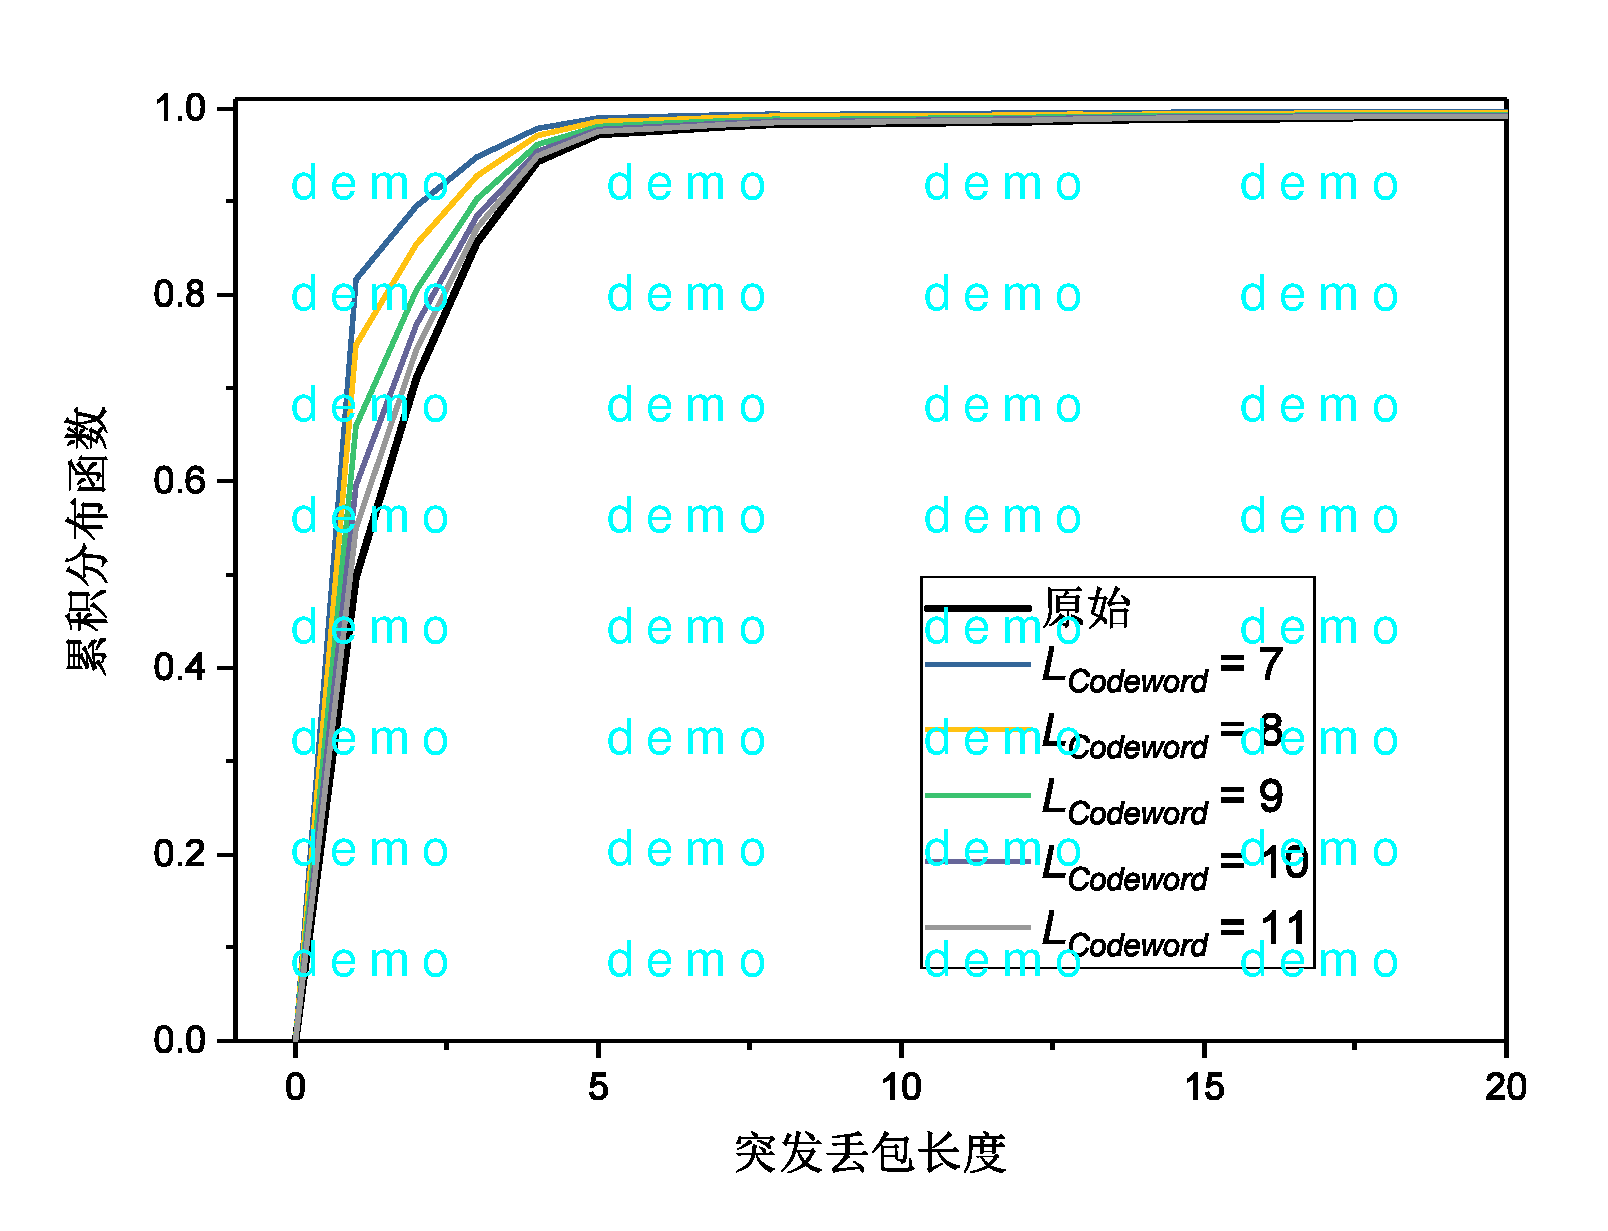
\includegraphics[width=0.48\textwidth]{chapters/chapter4/figures/burst-cdf-excellent.pdf}
        }
        \subfigure[Good场景的CDF]{
            \label{fig:4:results:burst:cdf:good}
            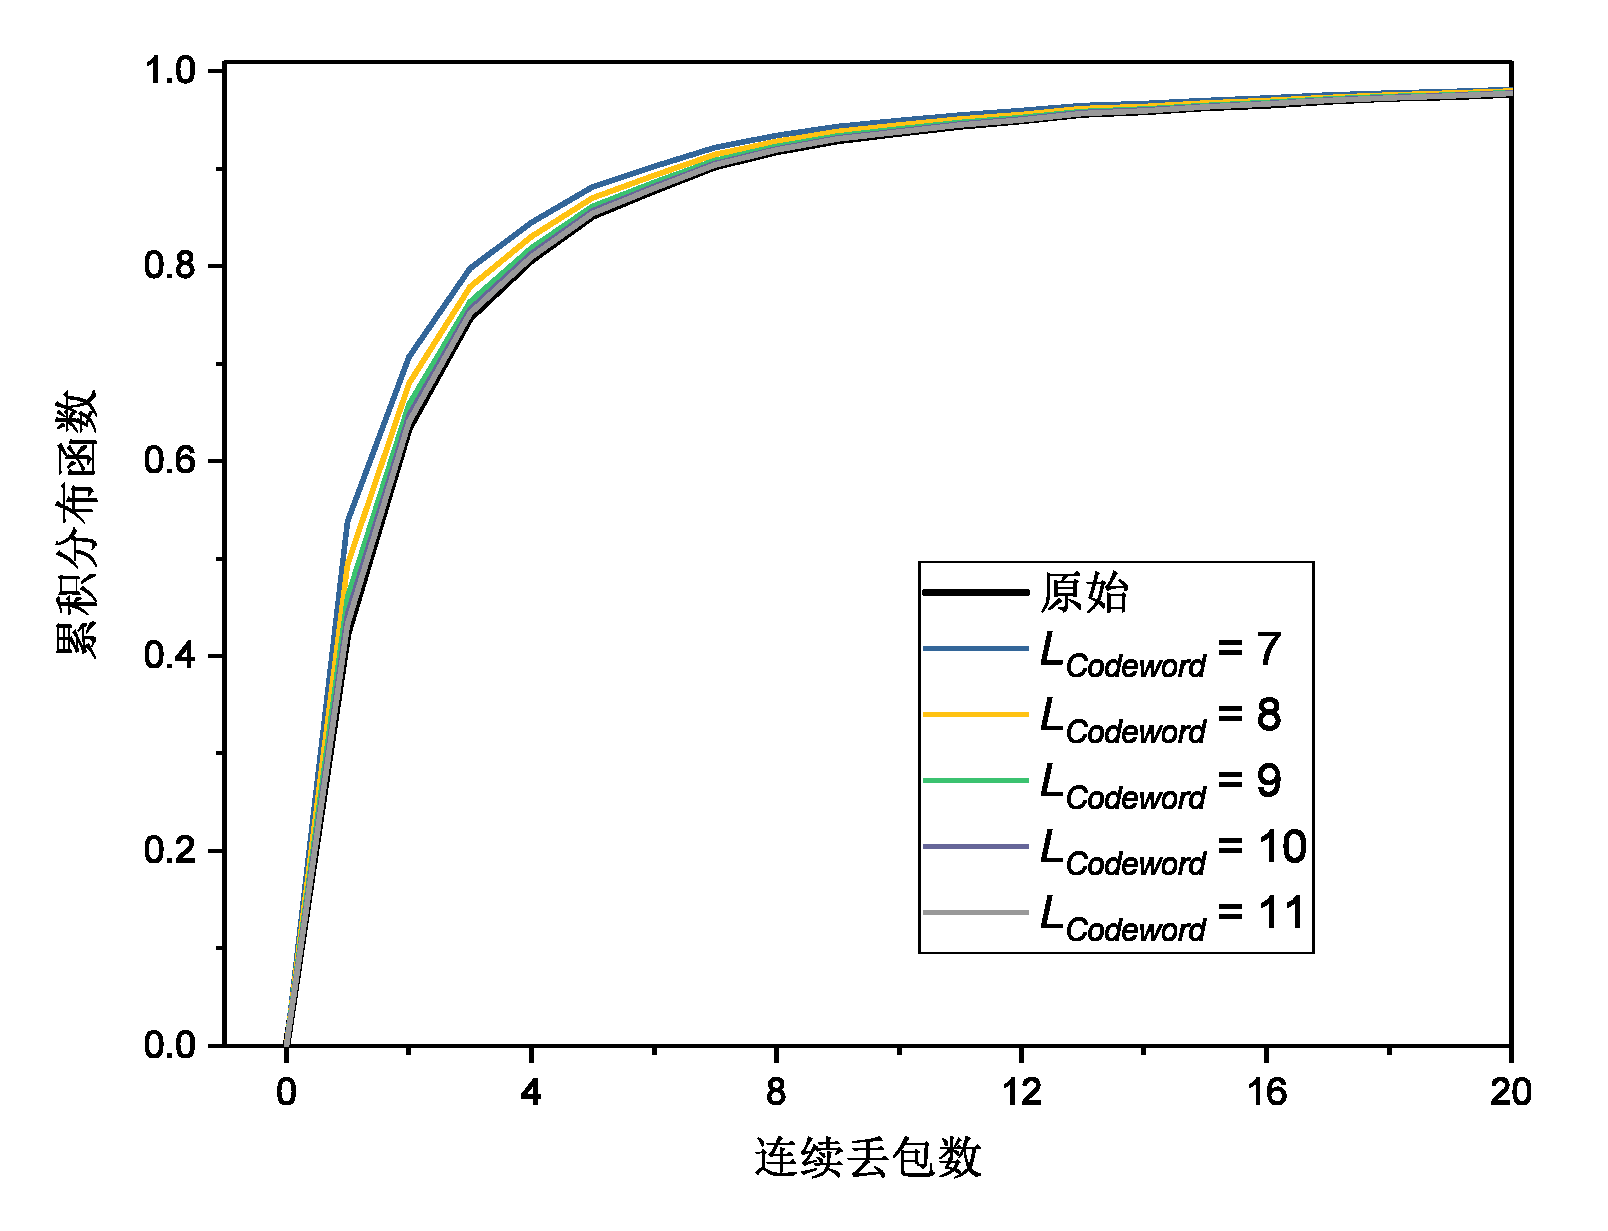
\includegraphics[width=0.48\textwidth]{chapters/chapter4/figures/burst-cdf-good.pdf}
        }
        \caption{突发丢包长度的CDF曲线}
        \label{fig:4:results:burst:cdf}
    \end{figure}
    
    \begin{figure}
        \centering
        \subfigure[窗口100时Excellent场景的CDF]{
            \label{fig:4:results:win100:cdf:excellent}
            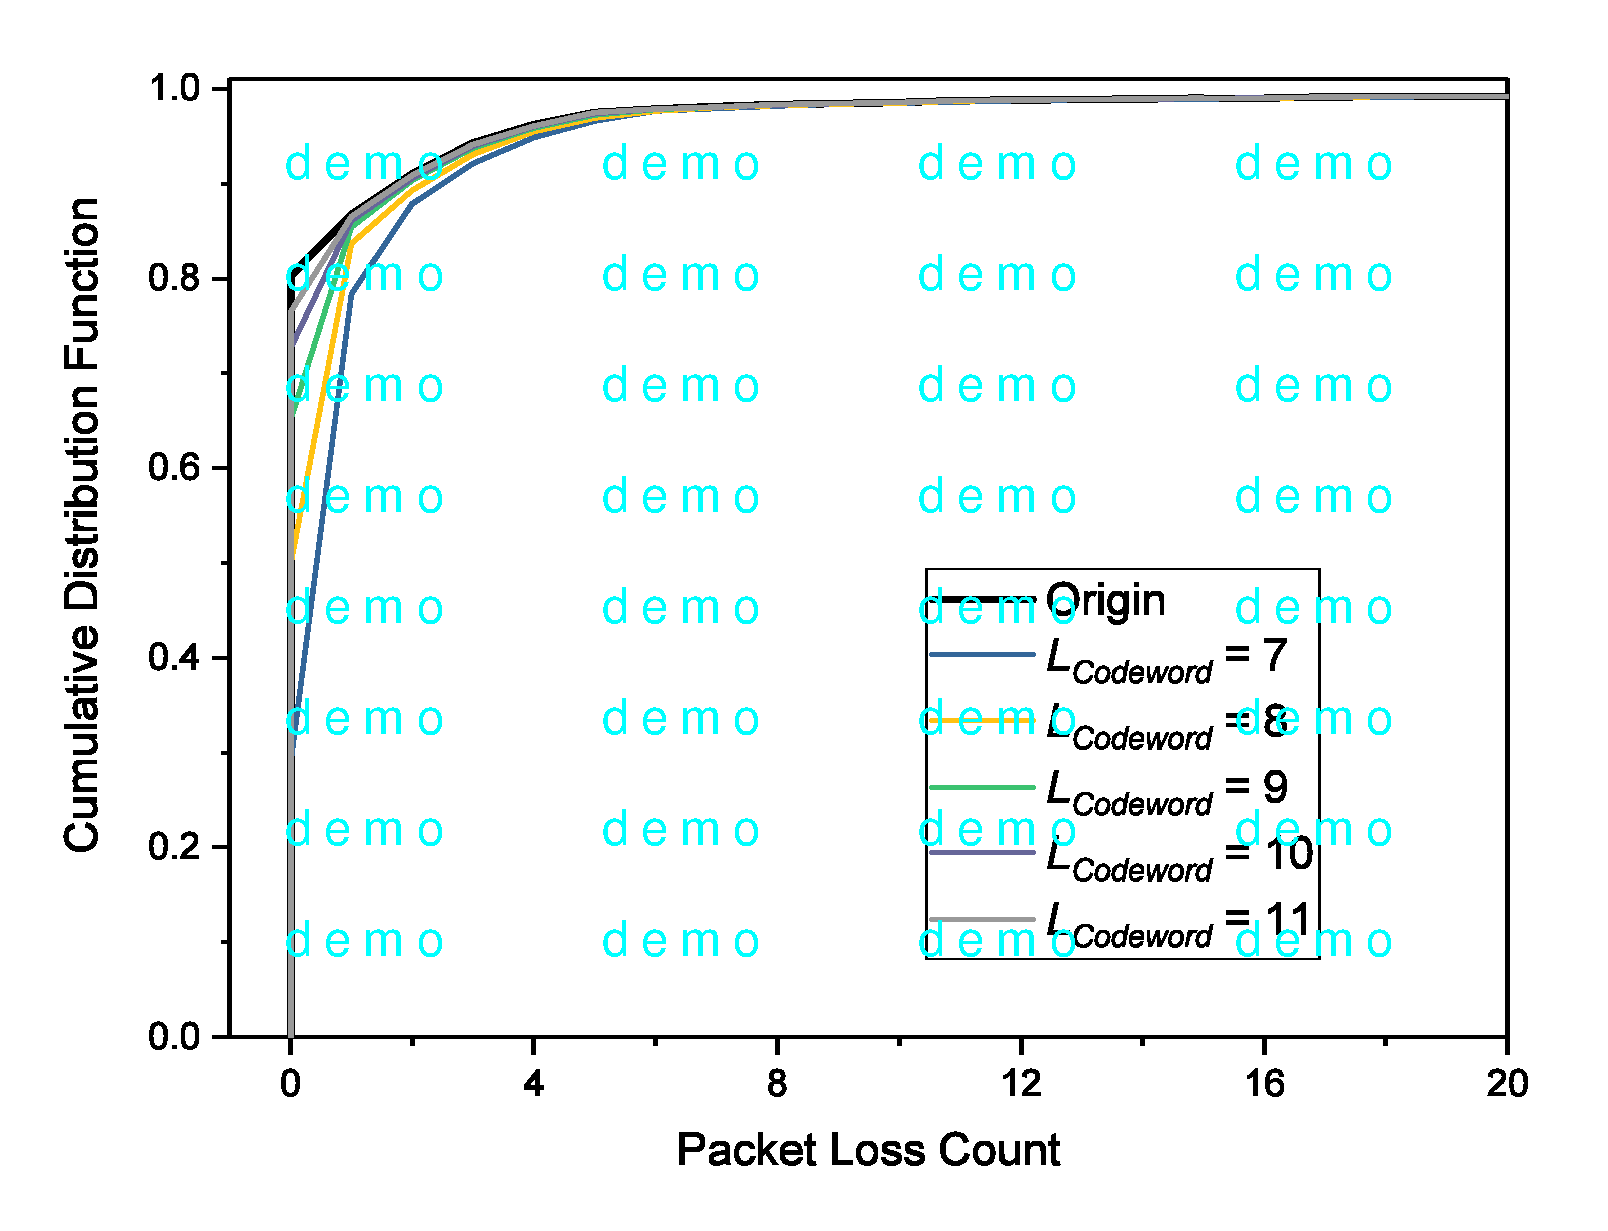
\includegraphics[width=0.48\textwidth]{chapters/chapter4/figures/win100-cdf-excellent.pdf}
        }
        \subfigure[窗口100时Good场景的CDF]{
            \label{fig:4:results:win100:cdf:good}
            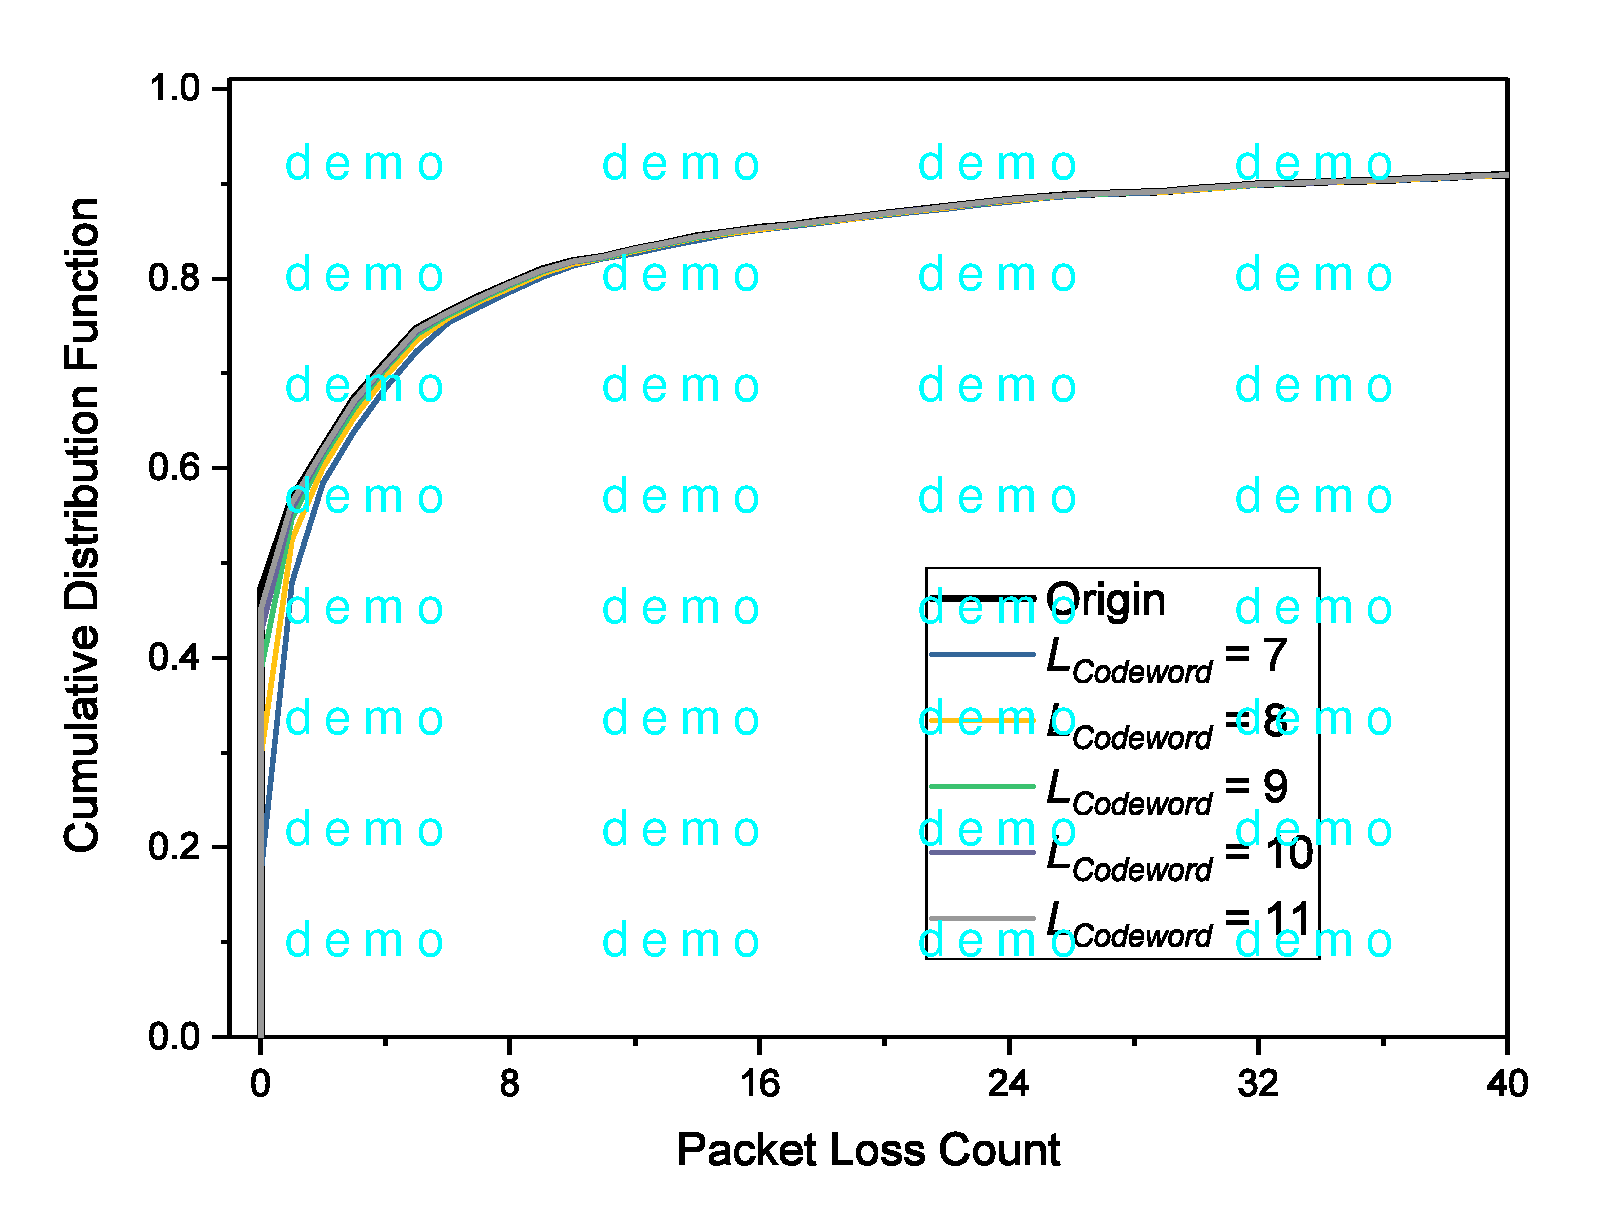
\includegraphics[width=0.48\textwidth]{chapters/chapter4/figures/win100-cdf-good.pdf}
        }
        \subfigure[窗口200时Excellent场景的CDF]{
            \label{fig:4:results:win200:cdf:excellent}
            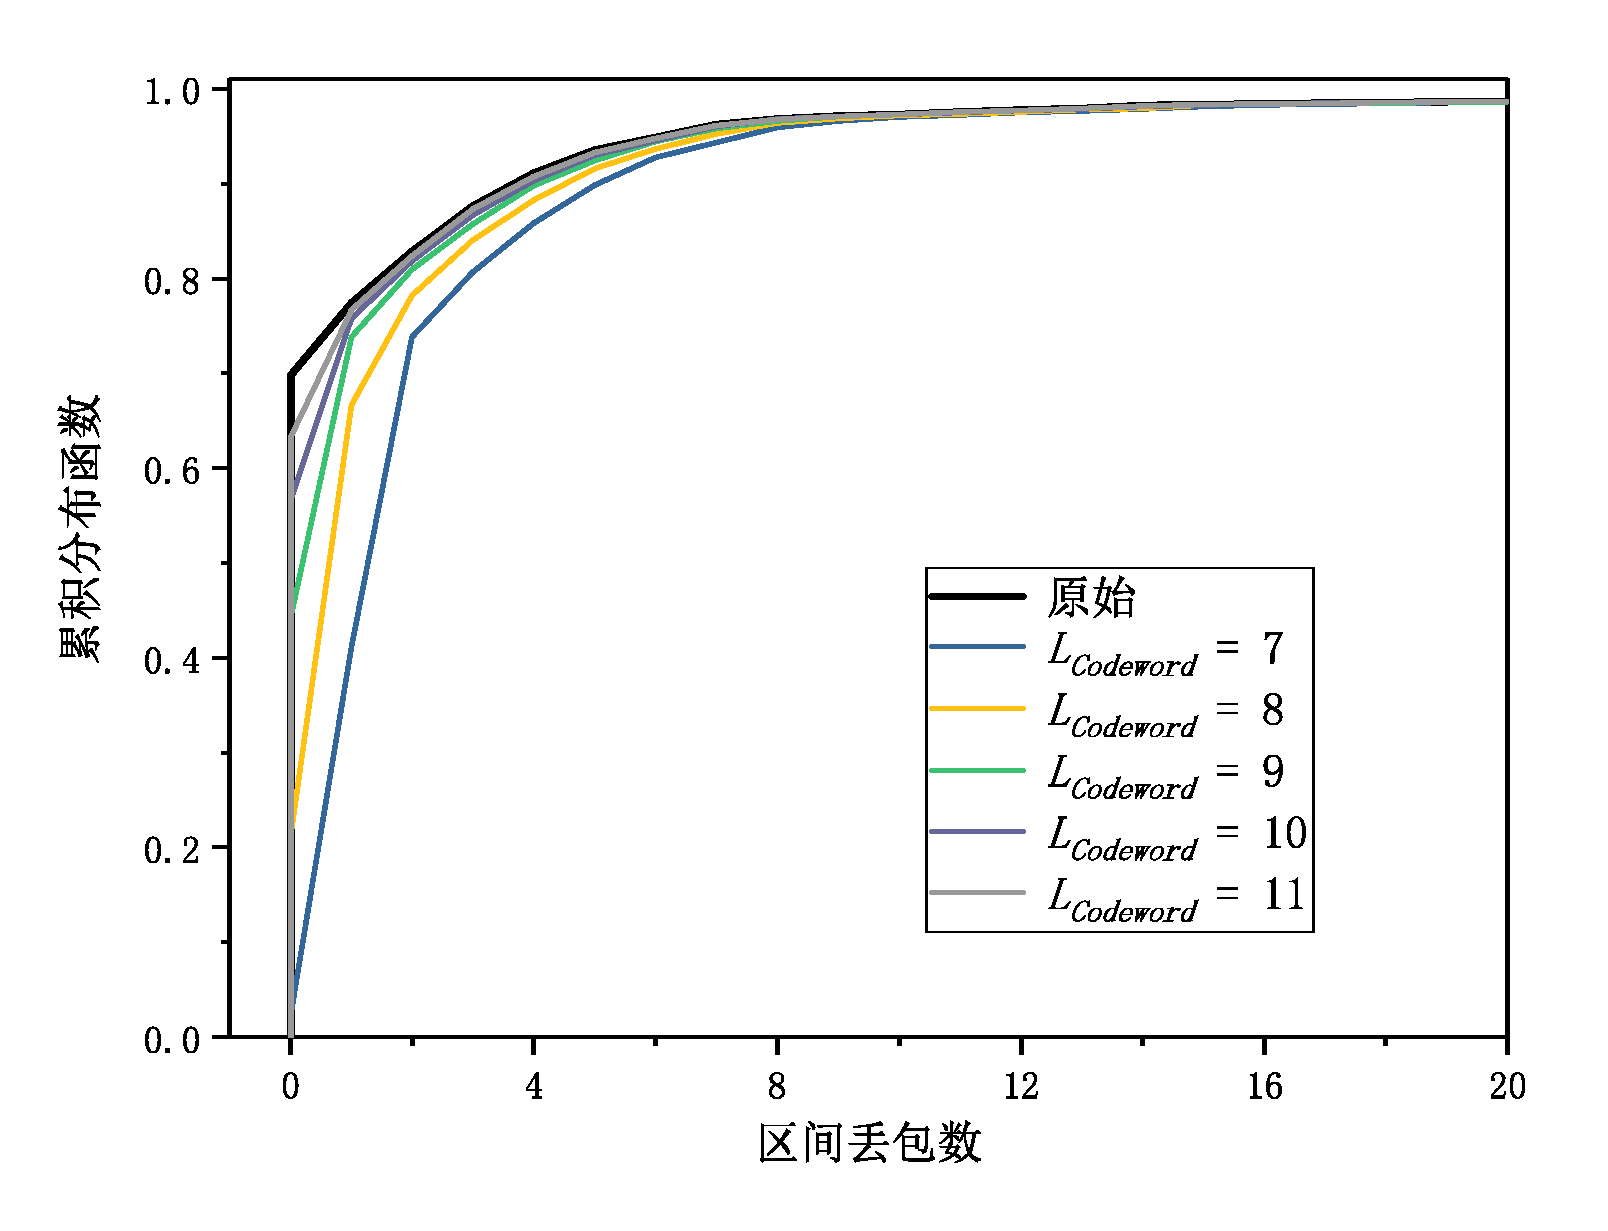
\includegraphics[width=0.48\textwidth]{chapters/chapter4/figures/win200-cdf-excellent.pdf}
        }
        \subfigure[窗口200时Good场景的CDF]{
            \label{fig:4:results:win200:cdf:good}
            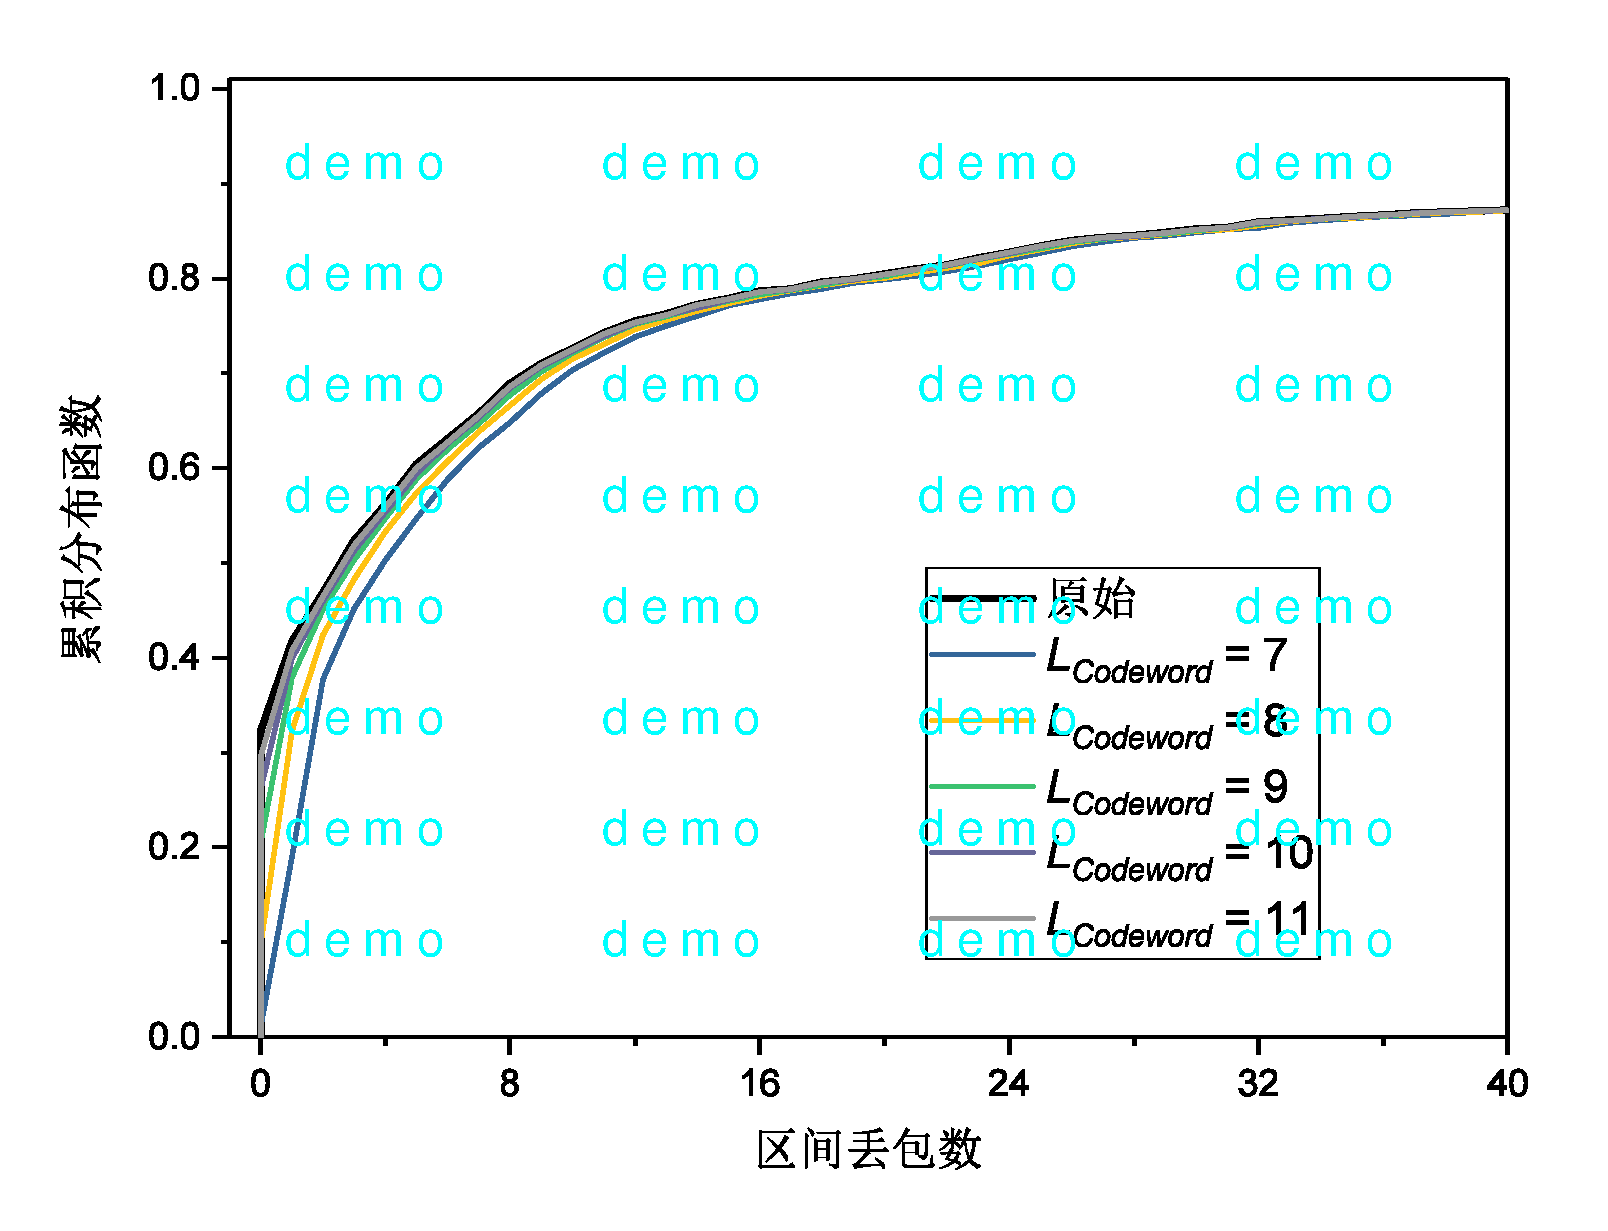
\includegraphics[width=0.48\textwidth]{chapters/chapter4/figures/win200-cdf-good.pdf}
        }
        \caption{区间丢包数的CDF曲线}
        \label{fig:4:results:win:cdf}
    \end{figure}
}

\subsubsection{IPD分布测试}
\label{chap:zigzag:results:undetectability:ipd}

\insertTable{
	\begin{table}[]
      \centering
      \caption{IPD分布测试检出率汇总表}
      \label{tab:4:results:ipd}
          \begin{tabular*}{0.75\textwidth}{@{\extracolsep{\fill}}ccc}
            \toprule
            $L_{Codeword}$ & 方法 & 检出率\\ 
            \midrule
            \multirow{5}{*}{7,8,9,10,11} 
            & K-S检验 & 0\% \\
            & T检验 \& Rank检验 & 0\% \\
            & K-L散度 & 0\% \\
            & Wasserstein距离 & 0\% \\
            & 能量距离 & 0\% \\
            \bottomrule
          \end{tabular*}
    \end{table}
}

IPD分布的CDF曲线如图\nref{fig:4:results:ipd:cdf}所示,在两种不同的场景中,IPD的分布已经无法区分该时间隐通道,CDF曲线已经高度趋于一致。该结果与\nref{chap:analyze:result:ipd:cdf}中的测试结果类似,当$L_{Codeword}\ge 7$时,在IPD分布上已经没有显著的差异,传统基于IPD的检测方法无法检测出该时间隐通道。

对IPD的量化检测结果如表\nref{tab:4:results:ipd},所有的参数在所有的场景中,均与原始分布保持高度一致,分布一致性检验无法检测出改时间隐通道。检测结果证明,该时间隐通道在IPD分布的检测中,具备抗检测能力,满足时间隐通道的隐蔽性要求。

\subsubsection{突发丢包长度测试}
\label{chap:zigzag:results:undetectability:burst}

\insertTable{
	\begin{table}[]
      \centering
      \caption{突发丢包长度测试检出率汇总表}
      \label{tab:4:results:burst}
          \begin{tabular*}{0.75\textwidth}{@{\extracolsep{\fill}}cccc}
            \toprule
            场景 & $L_{Codeword}$ & 方法 & 检出率 \\ 
            \midrule
            \multirow{4}{*}{Excellent} 
            & 7,8 & K-L散度 & 100\% \\
            & 9,10,11 & K-L散度 & 0\% \\
            & 7,8,9,10,11 & Wasserstein距离 & 0\% \\
            & 7,8,9,10,11 & 能量距离 & 0\% \\
            \\
            \multirow{3}{*}{Good}
            & 7,8,9,10,11 & K-L散度 & 0\% \\
            & 7,8,9,10,11 & Wasserstein距离 & 0\% \\
            & 7,8,9,10,11 & 能量距离 & 0\% \\
            \bottomrule
          \end{tabular*}
    \end{table}
}

不同参数下,突发丢包长度的累积分布函数曲线,如图\nref{fig:4:results:burst:cdf}。两种场景中,时间隐通道的曲线均出现了一定偏离,并且在Excellent场景中的差异更加明显。总体来说,随着$L_{Codeword}$的增大,时间隐通道的分布特征与原始分布更加接近,与理论预期一致。参照表\nref{tab:4:parameters},参数$L_{Codeword}$与调制产生的丢包率成反比,减少丢包则减弱对分布的影响。

不同场景中,对不同参数下的时间隐通道进行突发丢包长度检验,得到的结果如表\nref{tab:4:results:burst}。Excellent场景中,当$L_{Codeword}\ge 9$时,根据突发丢包长度的分布,已经无法区分时间隐通道与正常通道。Good场景中,基于主动丢包的时间隐通道与噪声分布相近,检测方法无法进行区分。因此,时间隐通道要通过突发丢包长度的检验,Excellent场景下$L_{Codeword}$至少为9,Good场景下$L_{Codeword}\ge 7$即可满足要求。

\subsubsection{区间丢包数测试}
\label{chap:zigzag:results:undetectability:win}

\insertTable{
	\begin{table}[]
      \centering
      \caption{区间丢包数测试检出率汇总表}
      \label{tab:4:results:win}
          \begin{tabular*}{0.75\textwidth}{@{\extracolsep{\fill}}cccc}
            \toprule
            场景 & $L_{Codeword}$ & 方法 & 检出率 \\ 
            \midrule
            \multirow{5}{*}{Excellent} 
            & 7,8,9,10,11 & K-L散度 & 0\% \\
            & 7 & Wasserstein距离 & 100\% \\
            & 8,9,10,11 & Wasserstein距离 & 0\% \\
            & 7 & 能量距离 & 100\% \\
            & 8,9,10,11 & 能量距离 & 0\% \\
            \\
            \multirow{7}{*}{Good}
            & 7,8,9,10,11 & K-L散度 & 0\% \\
            & 7 & Wasserstein距离 & 100\% \\
            & 8 & Wasserstein距离 & 30\% \\
            & 9,10,11 & Wasserstein距离 & 0\% \\
            & 7 & 能量距离 & 100\% \\
            & 8 & 能量距离 & 30\% \\
            & 9,10,11 & 能量距离 & 0\% \\
            \bottomrule
          \end{tabular*}
    \end{table}
}

在区间丢包数的测试中,采用的窗口长度与\nref{chap:analyze:result:window}保持一致,分别为100及200。区间丢包数的CDF曲线如图\nref{fig:4:results:win:cdf},与\nref{fig:3:result:win:cdf}不同的是,对基于Zigzag映射矩阵的时间隐通道的检测结果,CDF曲线起始位置没有发生明显的偏移,与\nref{chap:analyze:result:window}的检测结果基本一致。

对区间丢包数分布的量化评估结果,如表\nref{tab:4:results:win},K-L散度无法有效区分时间隐通道,而Wasserstein距离及能量距离具备一定的检测能力。Excellent场景下,当$L_{Codeword}\ge 8$时即可通过所有的测试;而在Good场景下,当$L_{Codeword}\ge 9$时才可以通过所有测试。

\subsubsection{抗检测能力测试汇总}
\label{chap:zigzag:results:undetectability:all}

\insertTable{
	\begin{table}[]
      \centering
      \caption{基于Zigzag映射矩阵的时间隐通道检出率汇总表}
      \label{tab:4:results:sum}
          \begin{tabular*}{0.8\textwidth}{@{\extracolsep{\fill}}cccccc}
            \toprule
            \multirow{2}{*}{场景} 
            & \multicolumn{5}{c}{$L_{Codeword}$} \\
            & 7 & 8 & 9 & 10 & 11 \\
            \midrule
            Excellent & 100\% & 100\% & 0\% & 0\% & 0\% \\
            Good & 100\% & 30\% & 0\% & 0\% & 0\% \\
            \bottomrule
          \end{tabular*}
    \end{table}
}

汇总所有的测试项目,基于Zigzag映射矩阵的时间隐通道,在抗检测能力测试中的最终结果如表\nref{tab:4:results:sum}。当$L_{Codeword}\ge 9$时,即可在所有场景中通过检测;当$L_{Codeword} = 8$时,在Good场景下有一定几率通过检测。通过对比可以发现,Excellent场景对主动丢包的容忍度有限,传输参数需要合理设置。

通过抗检测能力测试,基于Zigzag映射矩阵的时间隐通道,通过调整传输参数$L_{Codeword}$,在各种通话场景下均可通过测试。测试结果与表\nref{tab:3:result-sum:all}基本一致,可以同时验证该时间隐通道构建方法及时间隐通道检测方法。

\subsection{鲁棒性测试}
\label{chap:zigzag:results:robustness}

\insertFigure{
	\begin{figure}
        \centering
        \subfigure[Excellent及Good场景]{
            \label{fig:4:results:ber:scenario}
            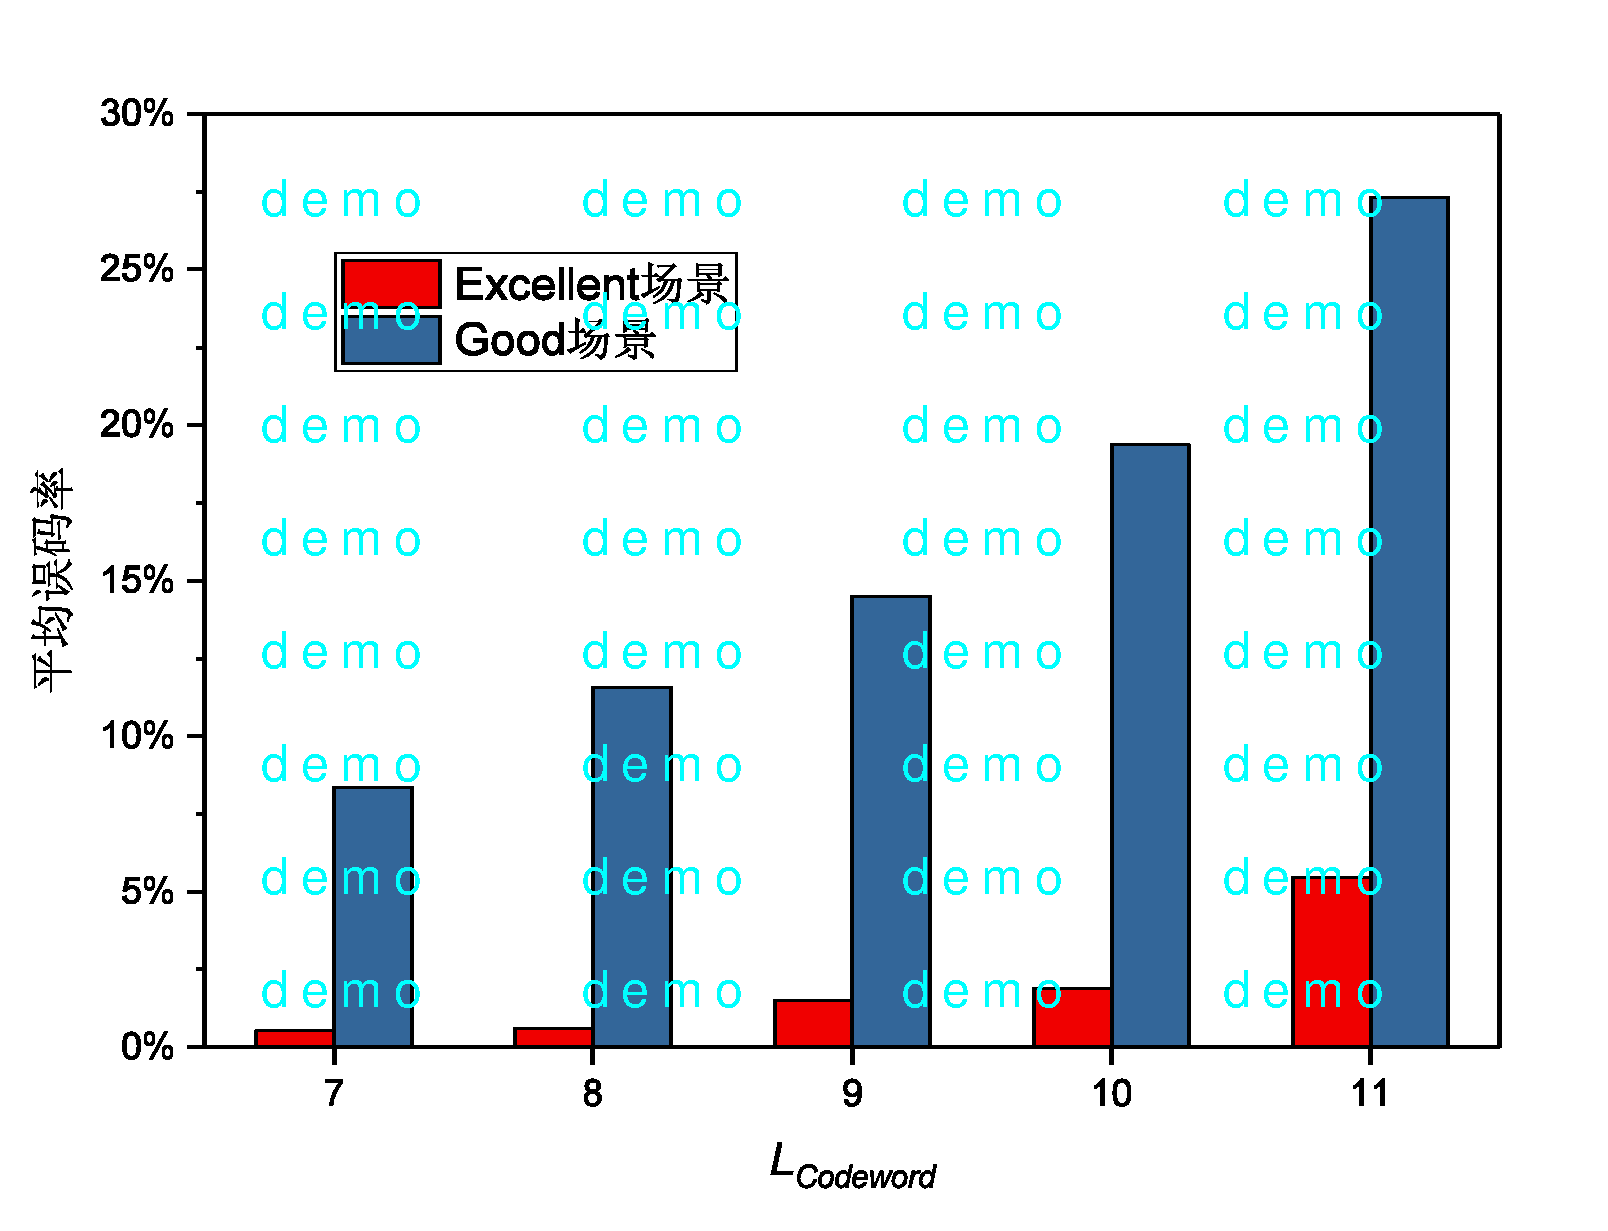
\includegraphics[width=0.48\textwidth]{chapters/chapter4/figures/ber-scenarios.pdf}
        }
        \subfigure[随机噪声场景]{
            \label{fig:4:results:ber:random}
            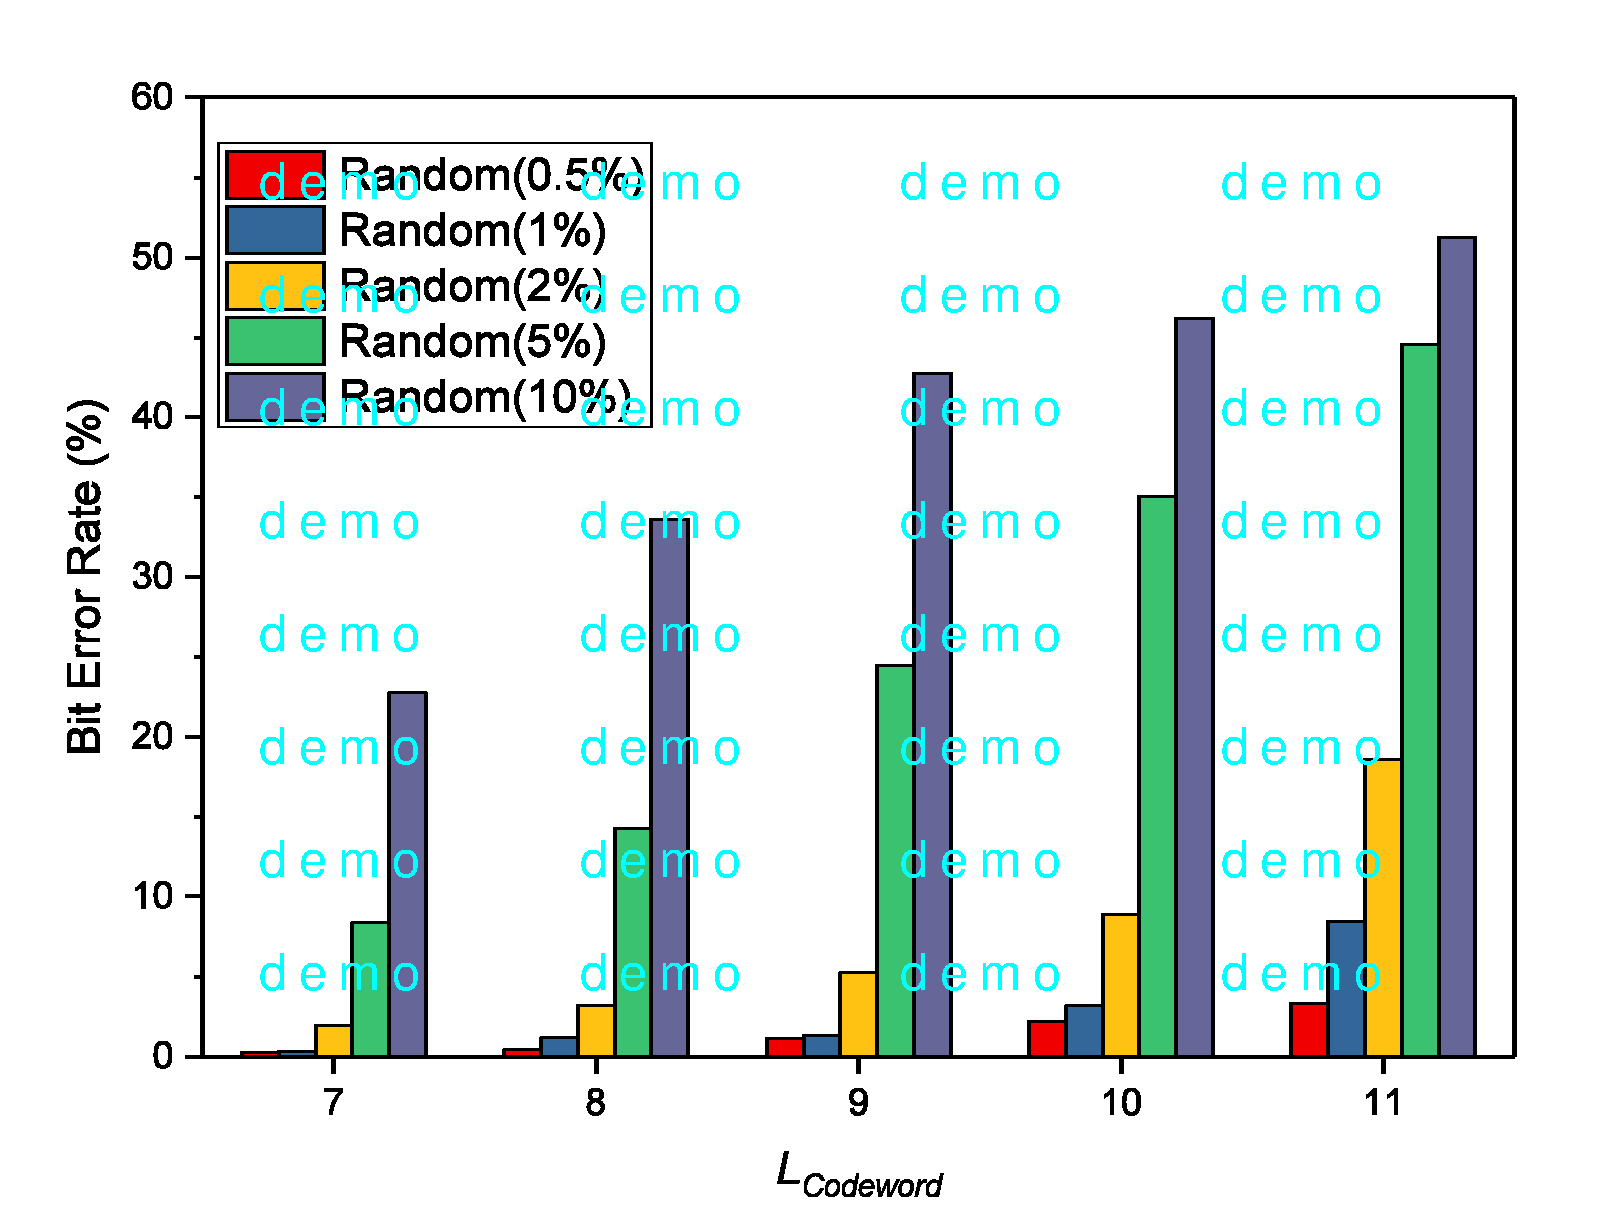
\includegraphics[width=0.48\textwidth]{chapters/chapter4/figures/ber-random.pdf}
        }
        \caption{时间隐通道的误码率水平}
        \label{fig:4:results:ber}
    \end{figure}
}

根据公式(\nref{equ:2:ber}),误码率也就是BER(Bit Error Rate)是评估鲁棒性的基本方式。为有效评估该时间隐通道,除了Excellent及Good两种测试场景,同时引入了具有不同丢包率的随机测试场景。最终各场景下的误码率水平如图\nref{fig:4:results:ber},其中图\nref{fig:4:results:ber:scenario}为抓包的Excellent及Good场景测试结果,图\nref{fig:4:results:ber:random}为随机噪声下的测试结果。

通过测试结果可发现,随着$L_{Codeword}$的增长,误码率水平显著增加。由于$L_{Codeword}$ bit的数据需要$2^{L_{Codeword}}$个数据包完成调制,因此增大$L_{Codeword}$导致区间内噪声产生的丢包数增加,码字鉴别的准确率降低,时间隐通道的鲁棒性减弱,误码率升高。

网络噪声,尤其是随机丢包对该时间隐通道的影响显著。Excellent场景中的传输可靠性,明显优于Good场景,传输结果基本满足传输需求;而Good场景中噪声干扰导致误码率过高,无法实现有效数据传输。对比图\nref{fig:4:results:ber:random}中随机噪声下的误码率,Excellent场景与$1\%$随机噪声的结果相近,Good场景与$10\%$随机噪声的结果相近,与抓包场景下的丢包率基本一致(表\nref{tab:3:capture-results})。对比结果表明,随机丢包是对基于主动丢包的时间隐通道鲁棒性的最大干扰,二者在表现及特征方面具有极高的相似度。

在满足抗检测性要求,即$L_{Codeword}\ge 9$的基础上,该时间隐通道在Excellent场景下可以保证$2\%$左右的误码率,在Good场景中误码率水平上升至$15\%$左右,对传输可靠性存在考验。因此,该时间隐通道构建方法,适应于无网络状况较好的场景,高丢包率场景下无法保证结果正确性。

\subsection{传输性能测试}
\label{chap:zigzag:results:throughput}

\insertTable{
	\begin{table}[]
      \centering
      \caption{基于Zigzag映射矩阵的时间隐通道传输性能}
      \label{tab:4:results:throughput}
          \begin{tabular*}{0.8\textwidth}{@{\extracolsep{\fill}}cccccc}
            \toprule
            \multirow{2}{*}{指标} 
            & \multicolumn{5}{c}{$L_{Codeword}$} \\
            & 7 & 8 & 9 & 10 & 11 \\
            \midrule
            Throughput\ (bps) & 2.73 & 1.56 & 0.88 & 0.49 & 0.27 \\
            Capacity\ (bpp) & 0.027 & 0.016 & 0.009 & 0.005 & 0.003 \\
            \bottomrule
          \end{tabular*}
    \end{table}
}

根据公式(\nref{equ:4:throughput}),该时间隐通道的传输性能只与参数$L_{Codeword}$有关。不同参数下的传输性能如表\nref{tab:4:results:throughput},传输性能与$L_{Codeword}$呈反比关系。在满足鲁棒性前提下,当$L_{Codeword}=9$时,达到最高性能0.88\ bps,增大$L_{Codeword}$导致性能按照$1/2$的比例依次衰减。

从传输性能的角度考虑,降低$L_{Codeword}$可以有效提升传输速率,但带来的代价是抗检测能力的衰退,违背了时间隐通道的研究前提。尤其是对基于主动丢包的时间隐通道来说,主动丢弃的数据包越多,对宿主信道意味着噪声越强,用户的通话质量将受到影响,同样影响隐通道的隐蔽性。

\subsection{构建代价测试}
\label{chap:zigzag:results:cost}

\insertFigure{
	\begin{figure}
        \centering
        \subfigure[Excellent场景的视频质量]{
            \label{fig:4:results:vq-excellent}
            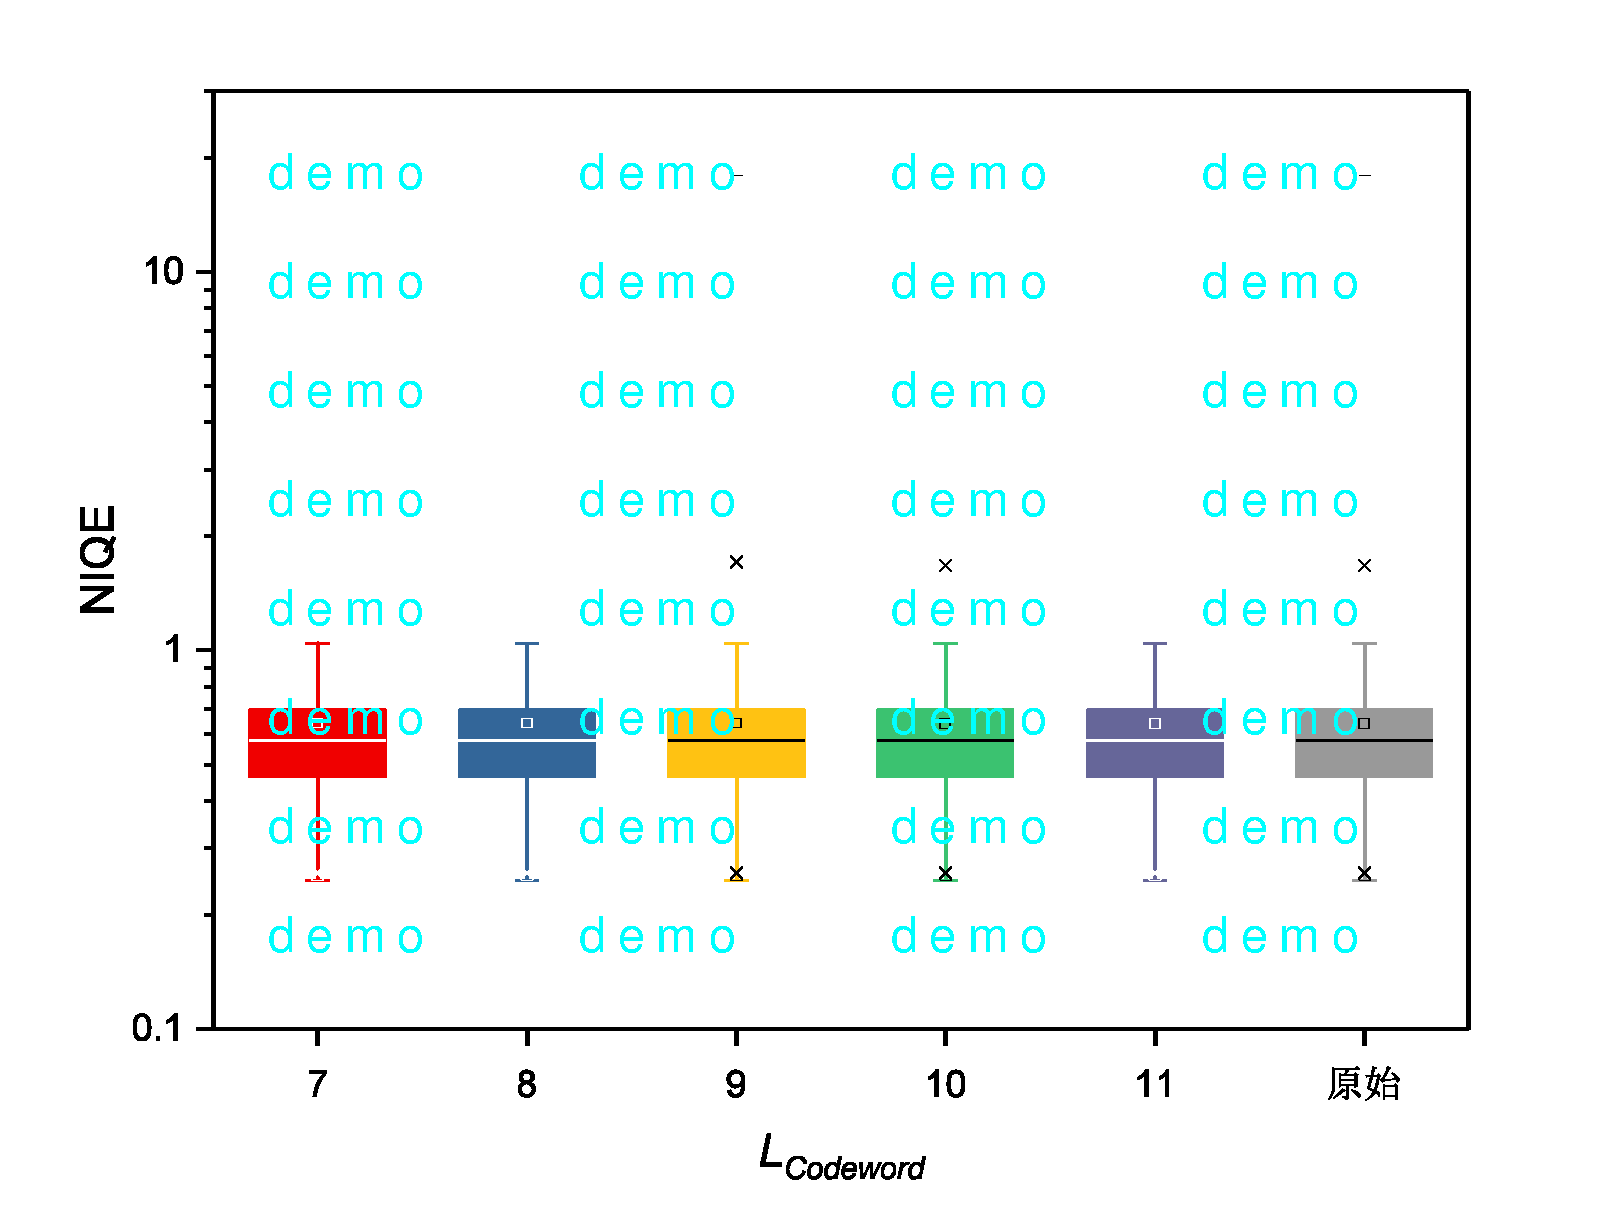
\includegraphics[width=0.48\textwidth]{chapters/chapter4/figures/vq-excellent.pdf}
        }
        \subfigure[Good场景的视频质量]{
            \label{fig:4:results:vq-good}
            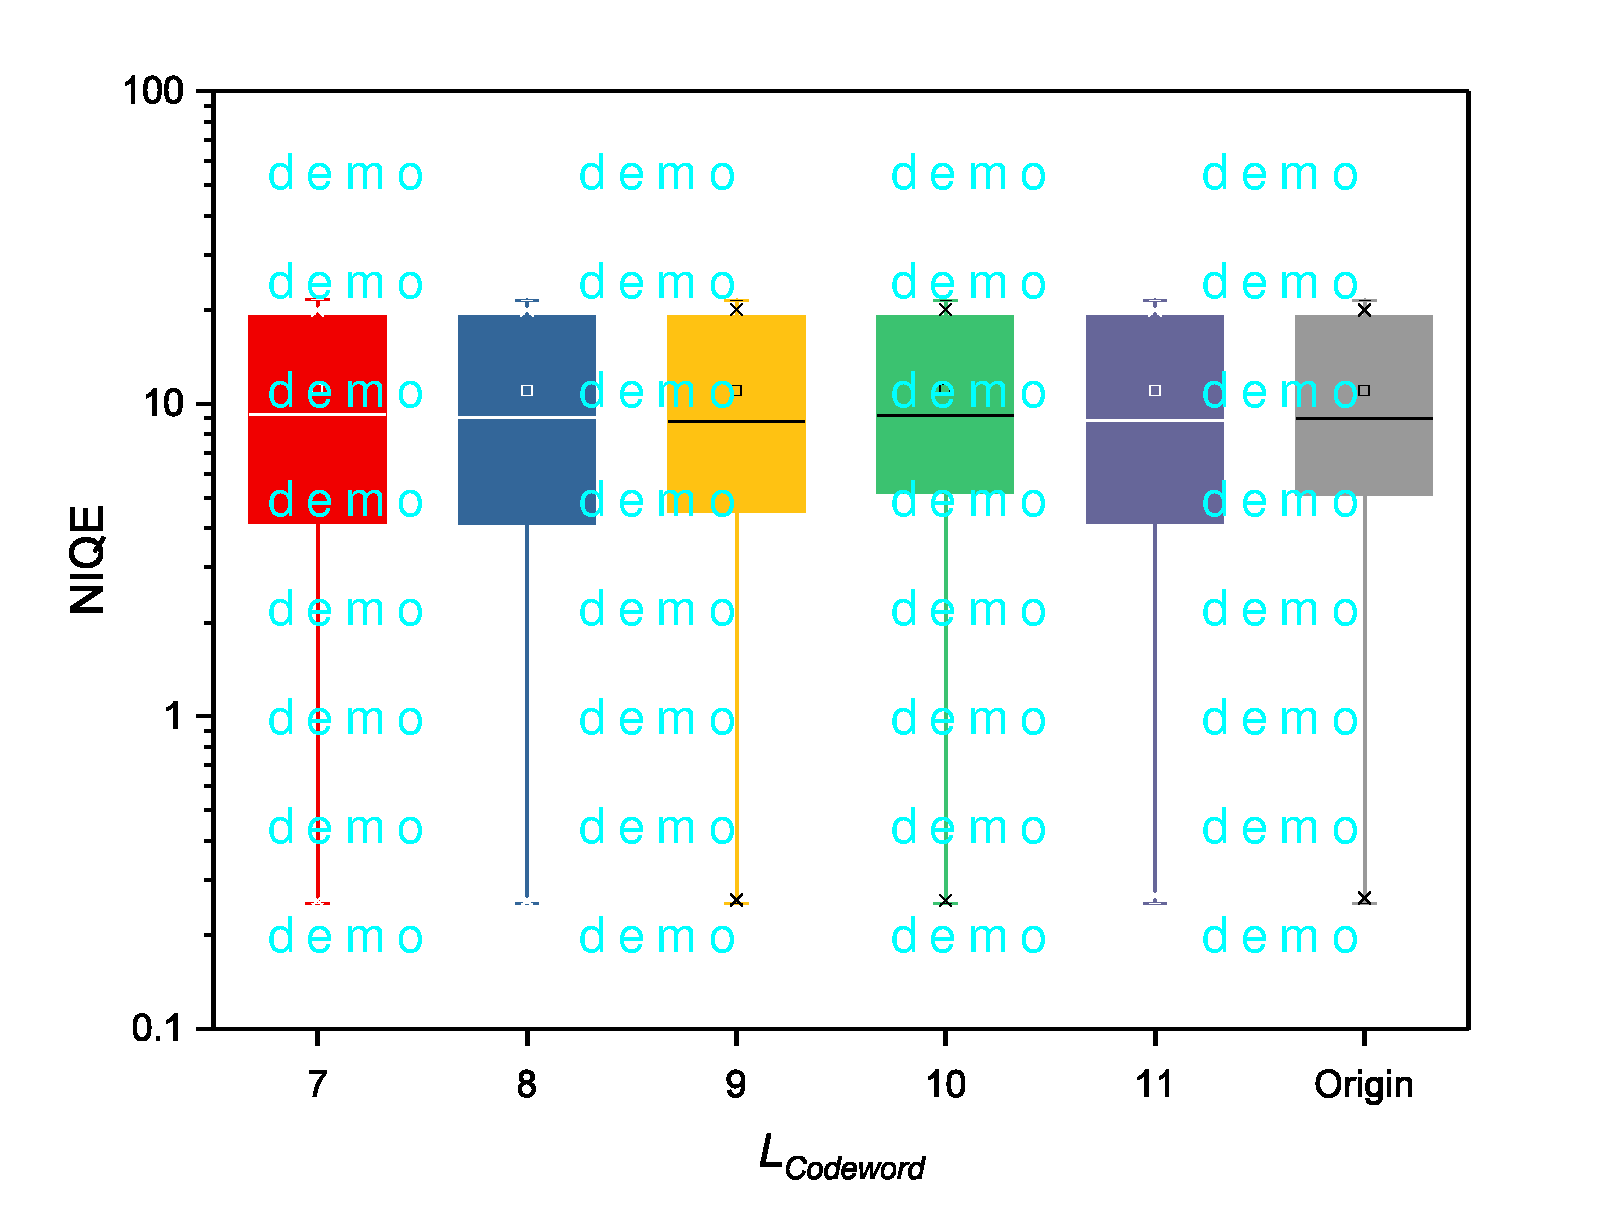
\includegraphics[width=0.48\textwidth]{chapters/chapter4/figures/vq-good.pdf}
        }
        \caption{时间隐通道的NIQE视频质量评估结果}
        \label{fig:4:results:vq}
    \end{figure}
}

基于Zigzag映射矩阵的时间隐通道,建立在VoLTE视频信道中,因此接收方的视频质量是评估构建代价的重要方面。根据表\nref{tab:4:parameters},当$L_{Codeword}\ge 9$时,构建时间隐通道导致的丢包率低于$0.2\%$,远小于网络噪声产生的丢包比例。

在视频质量方面,采用NIQE(Natural Image Quality Evaluator)无参照评价指标\nupcite{7094273},对视频中的所有帧进行质量评估,并判断视频整体的质量是否发生明显变化。\nupcite{7122356}NIQE反映了图像的失真程度,计算结果越大,证明图像质量越差。\nupcite{CoDLaCDAfMI,10.5120/ijca2017913550}两种场景下的视频质量评估结果如图\nref{fig:4:results:vq},Good场景下的NIQE值显著高于Excellent场景,证明Good场景下的通话体验受噪声干扰明显。

在两种场景中,对比NIQE图像质量的范围和均值,构建时间隐通道后没有发生明显的偏移。在Excellent场景中,NIQE值基本在1以下,得益于自身较好的传输质量,时间隐通道产生的影响在统计结果中无明显差异。Good场景中,原始的视频质量已经处于较差水平,时间隐通道导致NIQE值的范围和集中程度发生改变,但总体也没有出现明显的差异,统计结果基本一致。通过对比,本时间隐通道不会导致视频质量发生明显改变,满足时间隐通道低代价的要求。

\insertTable{
	\begin{table}[]
      \centering
      \caption{基于Zigzag映射矩阵的时间隐通道横向比较}
      \label{tab:4:results:compare}
          \begin{tabular*}{0.8\textwidth}{@{\extracolsep{\fill}}cccc}
            \toprule
            时间隐通道方法 & 性能 & 容量 & 误码率 \\
            \midrule
            SCC\nupcite{10.1007/978-3-642-16435-4_15} & & 0.2$\sim$ 0.8 bpp & 2\% \\
            AFTC\nupcite{7347395} & & 0.5 bpp & 4\% \\
            CoCo\nupcite{10.1007/978-3-642-24178-9_22} & & 0.1$\sim$ 0.5 bpp & 4\% \\
            SPCC\nupcite{8288828} & 0.7$\sim$ 3 bps & & 0.9\% \\
            Zigzag-CTC & 0.88 bps & 0.009 bpp & 1.5\% \\
            \bottomrule
          \end{tabular*}
    \end{table}
}

\subsection{结论}
\label{chap:zigzag:results:conclusion}

\insertFigure{
	\begin{figure}
        \centering
        \subfigure[Excellent场景下的综合评估]{
            \label{fig:4:results:sum:excellent}
            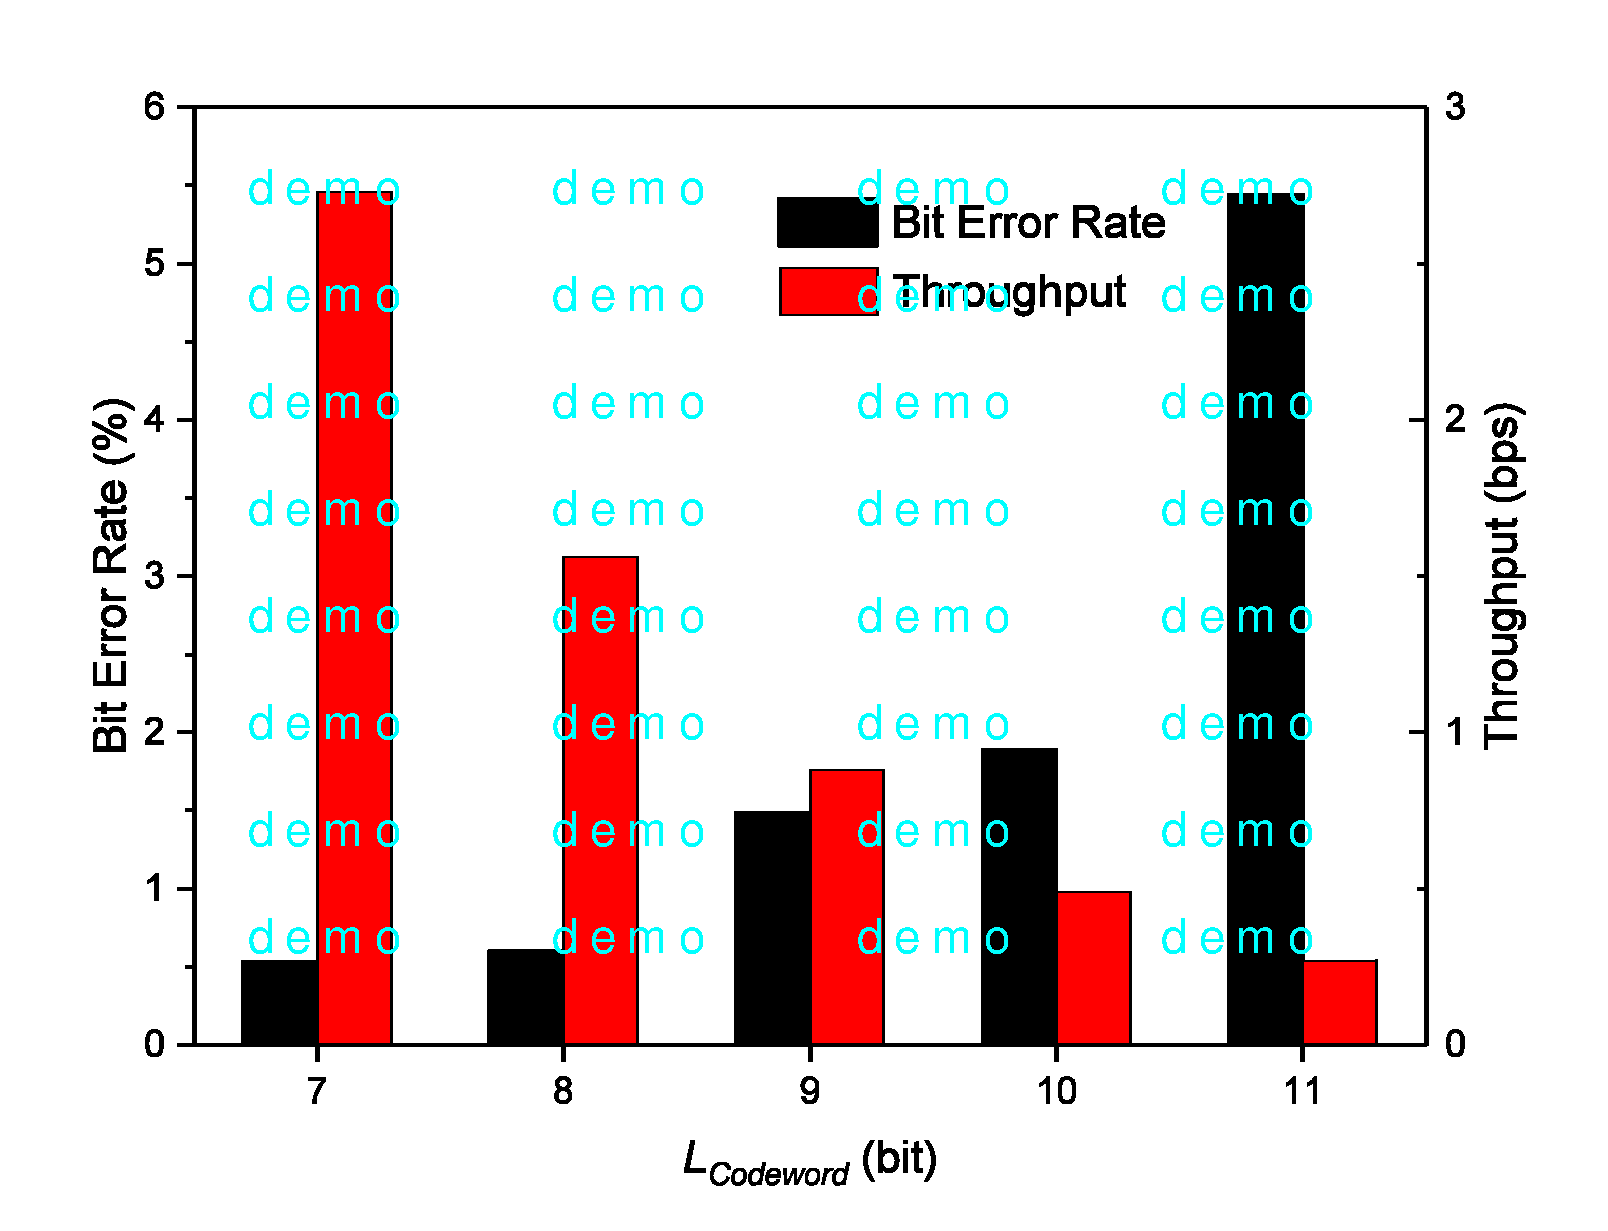
\includegraphics[width=0.48\textwidth]{chapters/chapter4/figures/sum-excellent.pdf}
        }
        \subfigure[Good场景下的综合评估]{
            \label{fig:4:results:sum:good}
            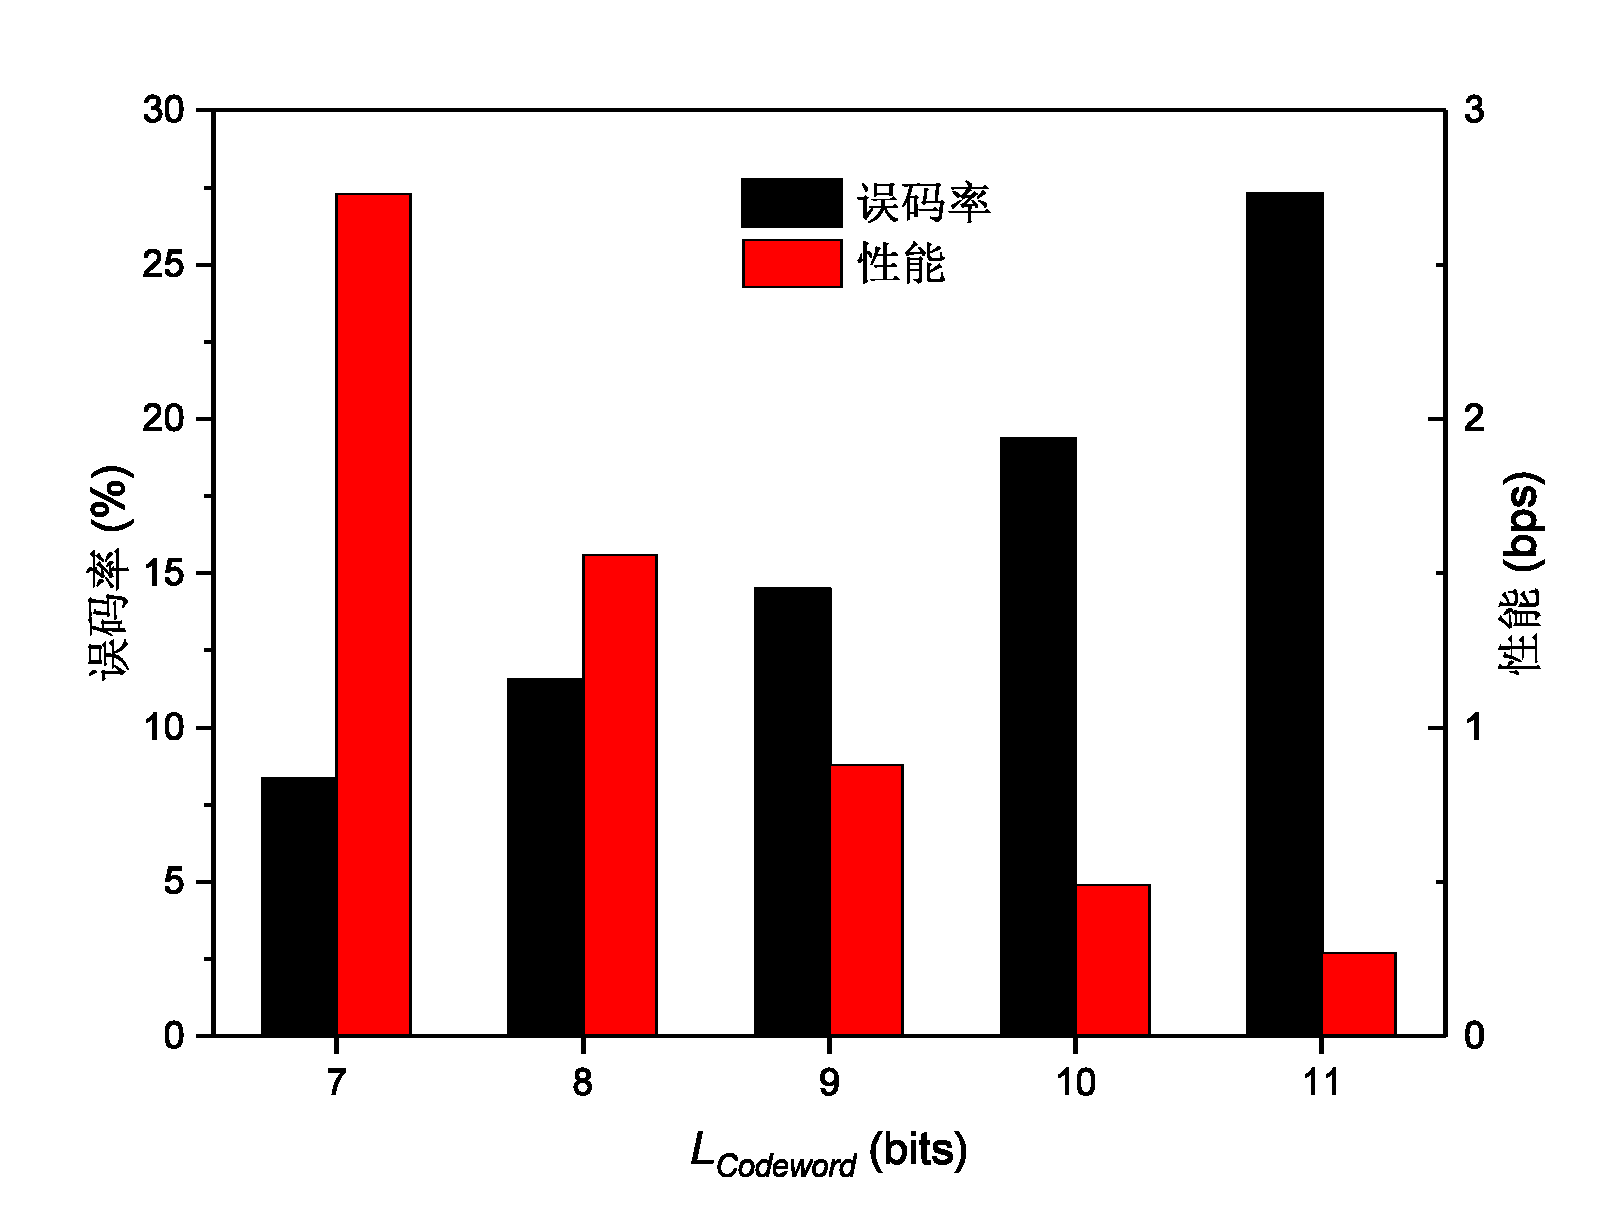
\includegraphics[width=0.48\textwidth]{chapters/chapter4/figures/sum-good.pdf}
        }
        \caption{基于Zigzag映射矩阵的时间隐通道综合评估}
        \label{fig:4:results:sum}
    \end{figure}
}

如图\nref{fig:4:results:sum},该时间隐通道的鲁棒性和传输性能,均具有$L_{Codeword}$越小结果越小的特点。结合\nref{chap:zigzag:results:undetectability}抗检测性评估结果,该时间隐通道的最优$L_{Codeword}$为9,在该参数下能够通过所有的检测方法,并且具有0.88bps的传输性能。

表\nref{tab:4:results:compare}对比了几种时间隐通道的性能及误码率水平,分别为SCC\nupcite{10.1007/978-3-642-16435-4_15}、AFTC\nupcite{7347395}、CoCo\nupcite{10.1007/978-3-642-24178-9_22}、SPCC\nupcite{8288828}及本时间隐通道构建方法Zigzag-CTC。由于宿主信道的区别,时间隐通道的信道容量存在差异,但在传输性能方面,该时间隐通道可以达到时间隐通道的基本水平。在鲁棒性方面,传输参数的设置会影响BER水平,该时间隐通道的最低误码率水平,与其它时间隐通道基本保持一致,满足应用要求。